% Created by tikzDevice version 0.12.3.1 on 2022-06-13 20:17:26
% !TEX encoding = UTF-8 Unicode
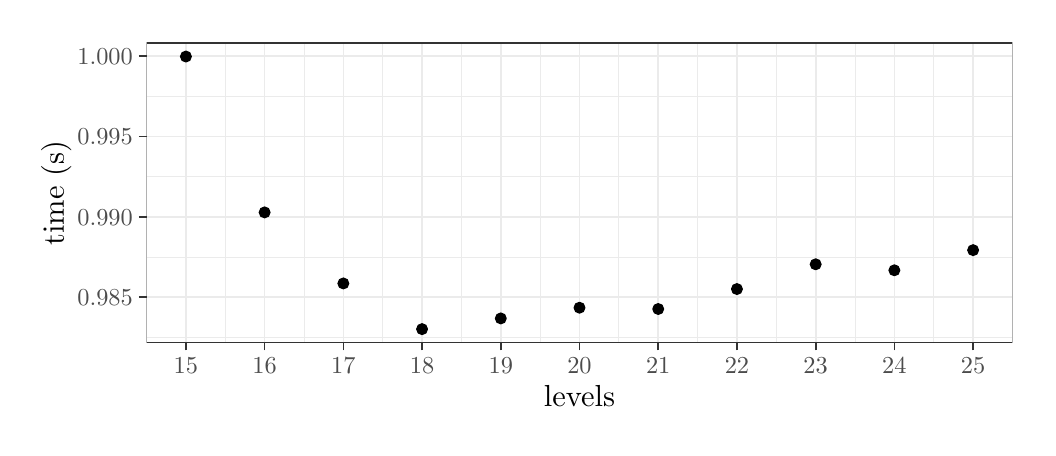
\begin{tikzpicture}[x=1pt,y=1pt]
\definecolor{fillColor}{RGB}{255,255,255}
\path[use as bounding box,fill=fillColor,fill opacity=0.00] (0,0) rectangle (361.35,144.54);
\begin{scope}
\path[clip] (  0.00,  0.00) rectangle (361.35,144.54);
\definecolor{drawColor}{RGB}{255,255,255}
\definecolor{fillColor}{RGB}{255,255,255}

\path[draw=drawColor,line width= 0.6pt,line join=round,line cap=round,fill=fillColor] (  0.00,  0.00) rectangle (361.35,144.54);
\end{scope}
\begin{scope}
\path[clip] ( 42.95, 30.69) rectangle (355.85,139.04);
\definecolor{fillColor}{RGB}{255,255,255}

\path[fill=fillColor] ( 42.95, 30.69) rectangle (355.85,139.04);
\definecolor{drawColor}{gray}{0.92}

\path[draw=drawColor,line width= 0.3pt,line join=round] ( 42.95, 32.62) --
	(355.85, 32.62);

\path[draw=drawColor,line width= 0.3pt,line join=round] ( 42.95, 61.67) --
	(355.85, 61.67);

\path[draw=drawColor,line width= 0.3pt,line join=round] ( 42.95, 90.71) --
	(355.85, 90.71);

\path[draw=drawColor,line width= 0.3pt,line join=round] ( 42.95,119.76) --
	(355.85,119.76);

\path[draw=drawColor,line width= 0.3pt,line join=round] ( 42.95, 30.69) --
	( 42.95,139.04);

\path[draw=drawColor,line width= 0.3pt,line join=round] ( 71.40, 30.69) --
	( 71.40,139.04);

\path[draw=drawColor,line width= 0.3pt,line join=round] ( 99.84, 30.69) --
	( 99.84,139.04);

\path[draw=drawColor,line width= 0.3pt,line join=round] (128.29, 30.69) --
	(128.29,139.04);

\path[draw=drawColor,line width= 0.3pt,line join=round] (156.73, 30.69) --
	(156.73,139.04);

\path[draw=drawColor,line width= 0.3pt,line join=round] (185.18, 30.69) --
	(185.18,139.04);

\path[draw=drawColor,line width= 0.3pt,line join=round] (213.62, 30.69) --
	(213.62,139.04);

\path[draw=drawColor,line width= 0.3pt,line join=round] (242.07, 30.69) --
	(242.07,139.04);

\path[draw=drawColor,line width= 0.3pt,line join=round] (270.51, 30.69) --
	(270.51,139.04);

\path[draw=drawColor,line width= 0.3pt,line join=round] (298.96, 30.69) --
	(298.96,139.04);

\path[draw=drawColor,line width= 0.3pt,line join=round] (327.40, 30.69) --
	(327.40,139.04);

\path[draw=drawColor,line width= 0.3pt,line join=round] (355.85, 30.69) --
	(355.85,139.04);

\path[draw=drawColor,line width= 0.6pt,line join=round] ( 42.95, 47.15) --
	(355.85, 47.15);

\path[draw=drawColor,line width= 0.6pt,line join=round] ( 42.95, 76.19) --
	(355.85, 76.19);

\path[draw=drawColor,line width= 0.6pt,line join=round] ( 42.95,105.24) --
	(355.85,105.24);

\path[draw=drawColor,line width= 0.6pt,line join=round] ( 42.95,134.28) --
	(355.85,134.28);

\path[draw=drawColor,line width= 0.6pt,line join=round] ( 57.18, 30.69) --
	( 57.18,139.04);

\path[draw=drawColor,line width= 0.6pt,line join=round] ( 85.62, 30.69) --
	( 85.62,139.04);

\path[draw=drawColor,line width= 0.6pt,line join=round] (114.07, 30.69) --
	(114.07,139.04);

\path[draw=drawColor,line width= 0.6pt,line join=round] (142.51, 30.69) --
	(142.51,139.04);

\path[draw=drawColor,line width= 0.6pt,line join=round] (170.96, 30.69) --
	(170.96,139.04);

\path[draw=drawColor,line width= 0.6pt,line join=round] (199.40, 30.69) --
	(199.40,139.04);

\path[draw=drawColor,line width= 0.6pt,line join=round] (227.85, 30.69) --
	(227.85,139.04);

\path[draw=drawColor,line width= 0.6pt,line join=round] (256.29, 30.69) --
	(256.29,139.04);

\path[draw=drawColor,line width= 0.6pt,line join=round] (284.74, 30.69) --
	(284.74,139.04);

\path[draw=drawColor,line width= 0.6pt,line join=round] (313.18, 30.69) --
	(313.18,139.04);

\path[draw=drawColor,line width= 0.6pt,line join=round] (341.63, 30.69) --
	(341.63,139.04);
\definecolor{drawColor}{RGB}{0,0,0}
\definecolor{fillColor}{RGB}{0,0,0}

\path[draw=drawColor,line width= 0.4pt,line join=round,line cap=round,fill=fillColor] ( 57.18,134.11) circle (  1.96);

\path[draw=drawColor,line width= 0.4pt,line join=round,line cap=round,fill=fillColor] ( 85.62, 77.79) circle (  1.96);

\path[draw=drawColor,line width= 0.4pt,line join=round,line cap=round,fill=fillColor] (114.07, 52.12) circle (  1.96);

\path[draw=drawColor,line width= 0.4pt,line join=round,line cap=round,fill=fillColor] (142.51, 35.61) circle (  1.96);

\path[draw=drawColor,line width= 0.4pt,line join=round,line cap=round,fill=fillColor] (170.96, 39.48) circle (  1.96);

\path[draw=drawColor,line width= 0.4pt,line join=round,line cap=round,fill=fillColor] (199.40, 43.35) circle (  1.96);

\path[draw=drawColor,line width= 0.4pt,line join=round,line cap=round,fill=fillColor] (227.85, 42.88) circle (  1.96);

\path[draw=drawColor,line width= 0.4pt,line join=round,line cap=round,fill=fillColor] (256.29, 50.09) circle (  1.96);

\path[draw=drawColor,line width= 0.4pt,line join=round,line cap=round,fill=fillColor] (284.74, 59.04) circle (  1.96);

\path[draw=drawColor,line width= 0.4pt,line join=round,line cap=round,fill=fillColor] (313.18, 56.87) circle (  1.96);

\path[draw=drawColor,line width= 0.4pt,line join=round,line cap=round,fill=fillColor] (341.63, 64.15) circle (  1.96);
\definecolor{drawColor}{gray}{0.20}

\path[draw=drawColor,line width= 0.6pt,line join=round,line cap=round] ( 42.95, 30.69) rectangle (355.85,139.04);
\end{scope}
\begin{scope}
\path[clip] (  0.00,  0.00) rectangle (361.35,144.54);
\definecolor{drawColor}{gray}{0.30}

\node[text=drawColor,anchor=base east,inner sep=0pt, outer sep=0pt, scale=  0.88] at ( 38.00, 44.12) {0.985};

\node[text=drawColor,anchor=base east,inner sep=0pt, outer sep=0pt, scale=  0.88] at ( 38.00, 73.16) {0.990};

\node[text=drawColor,anchor=base east,inner sep=0pt, outer sep=0pt, scale=  0.88] at ( 38.00,102.21) {0.995};

\node[text=drawColor,anchor=base east,inner sep=0pt, outer sep=0pt, scale=  0.88] at ( 38.00,131.25) {1.000};
\end{scope}
\begin{scope}
\path[clip] (  0.00,  0.00) rectangle (361.35,144.54);
\definecolor{drawColor}{gray}{0.20}

\path[draw=drawColor,line width= 0.6pt,line join=round] ( 40.20, 47.15) --
	( 42.95, 47.15);

\path[draw=drawColor,line width= 0.6pt,line join=round] ( 40.20, 76.19) --
	( 42.95, 76.19);

\path[draw=drawColor,line width= 0.6pt,line join=round] ( 40.20,105.24) --
	( 42.95,105.24);

\path[draw=drawColor,line width= 0.6pt,line join=round] ( 40.20,134.28) --
	( 42.95,134.28);
\end{scope}
\begin{scope}
\path[clip] (  0.00,  0.00) rectangle (361.35,144.54);
\definecolor{drawColor}{gray}{0.20}

\path[draw=drawColor,line width= 0.6pt,line join=round] ( 57.18, 27.94) --
	( 57.18, 30.69);

\path[draw=drawColor,line width= 0.6pt,line join=round] ( 85.62, 27.94) --
	( 85.62, 30.69);

\path[draw=drawColor,line width= 0.6pt,line join=round] (114.07, 27.94) --
	(114.07, 30.69);

\path[draw=drawColor,line width= 0.6pt,line join=round] (142.51, 27.94) --
	(142.51, 30.69);

\path[draw=drawColor,line width= 0.6pt,line join=round] (170.96, 27.94) --
	(170.96, 30.69);

\path[draw=drawColor,line width= 0.6pt,line join=round] (199.40, 27.94) --
	(199.40, 30.69);

\path[draw=drawColor,line width= 0.6pt,line join=round] (227.85, 27.94) --
	(227.85, 30.69);

\path[draw=drawColor,line width= 0.6pt,line join=round] (256.29, 27.94) --
	(256.29, 30.69);

\path[draw=drawColor,line width= 0.6pt,line join=round] (284.74, 27.94) --
	(284.74, 30.69);

\path[draw=drawColor,line width= 0.6pt,line join=round] (313.18, 27.94) --
	(313.18, 30.69);

\path[draw=drawColor,line width= 0.6pt,line join=round] (341.63, 27.94) --
	(341.63, 30.69);
\end{scope}
\begin{scope}
\path[clip] (  0.00,  0.00) rectangle (361.35,144.54);
\definecolor{drawColor}{gray}{0.30}

\node[text=drawColor,anchor=base,inner sep=0pt, outer sep=0pt, scale=  0.88] at ( 57.18, 19.68) {15};

\node[text=drawColor,anchor=base,inner sep=0pt, outer sep=0pt, scale=  0.88] at ( 85.62, 19.68) {16};

\node[text=drawColor,anchor=base,inner sep=0pt, outer sep=0pt, scale=  0.88] at (114.07, 19.68) {17};

\node[text=drawColor,anchor=base,inner sep=0pt, outer sep=0pt, scale=  0.88] at (142.51, 19.68) {18};

\node[text=drawColor,anchor=base,inner sep=0pt, outer sep=0pt, scale=  0.88] at (170.96, 19.68) {19};

\node[text=drawColor,anchor=base,inner sep=0pt, outer sep=0pt, scale=  0.88] at (199.40, 19.68) {20};

\node[text=drawColor,anchor=base,inner sep=0pt, outer sep=0pt, scale=  0.88] at (227.85, 19.68) {21};

\node[text=drawColor,anchor=base,inner sep=0pt, outer sep=0pt, scale=  0.88] at (256.29, 19.68) {22};

\node[text=drawColor,anchor=base,inner sep=0pt, outer sep=0pt, scale=  0.88] at (284.74, 19.68) {23};

\node[text=drawColor,anchor=base,inner sep=0pt, outer sep=0pt, scale=  0.88] at (313.18, 19.68) {24};

\node[text=drawColor,anchor=base,inner sep=0pt, outer sep=0pt, scale=  0.88] at (341.63, 19.68) {25};
\end{scope}
\begin{scope}
\path[clip] (  0.00,  0.00) rectangle (361.35,144.54);
\definecolor{drawColor}{RGB}{0,0,0}

\node[text=drawColor,anchor=base,inner sep=0pt, outer sep=0pt, scale=  1.10] at (199.40,  7.64) {levels};
\end{scope}
\begin{scope}
\path[clip] (  0.00,  0.00) rectangle (361.35,144.54);
\definecolor{drawColor}{RGB}{0,0,0}

\node[text=drawColor,rotate= 90.00,anchor=base,inner sep=0pt, outer sep=0pt, scale=  1.10] at ( 13.08, 84.86) {time (s)};
\end{scope}
\end{tikzpicture}
